\documentclass[10pt,a4paper]{article}
\usepackage[utf8]{inputenc}
\usepackage{amsmath}
\usepackage{amsfonts}
\usepackage{amssymb}
\usepackage{geometry}
\usepackage{verbatim}
\usepackage{enumerate}
\usepackage{fancyvrb}
\usepackage{graphicx}
\usepackage{tikz}
\usepackage{hyperref}
\usetikzlibrary{positioning}
\usetikzlibrary{shapes,snakes}
\usepackage[english]{babel}

\geometry{legalpaper, margin=1.5in}

\author{William Schultz}
\begin{document}
\title{Program Synthesis}
\author{William Schultz}
\maketitle

% \section{Reactive synthesis}

\begin{itemize}
    \item The \textbf{verification problem}: given system $M$ and spec $\varphi$, check that $M \vDash \varphi$.
    \item The \textbf{synthesis problem}: given spec $\varphi$, find $M$ such that $M \vDash \varphi$.
\end{itemize}

\subsection*{Deductive Synthesis}

The \textit{deductive approach} \cite{manna1980deductive} tries to synthesize an input/output program by extracting it from a realizability proof.

\subsection*{Temporal Synthesis}

\textit{Temporal synthesis} considers specifications given in the form of LTL (or CTL), for example. Initial approach was to use satisfiability of a temporal formula as a way to derive $M$ \cite{1981clarkemerson}. 
See also \cite{1984mannawolper}. 

In \cite{1981clarkemerson} they consider concurrent systems consisting of a finite number of fixed processes $P_1,\dots,P_m$ running in parallel. They treat parallelism in the usual sense i.e. non-deterministic interleaving of the sequential atomic actions of each process. They use CTL as a specification language, and consider the semantics of CTL with respect to a (Kripke) structure $M=(S,A_1,\dots,A_k,L)$, where
\begin{itemize}
    \item $S$: countable set of system states
    \item $A_i \subseteq S \times S$: transition relation of process $i$
    \item $L$: assignment of atomic propositions to each state
\end{itemize}
They use a decision procedure for satisfiability of CTL formulae (similar to one described in \cite{1981benari}) as part of their synthesis procedure. Given a CTL formula $f_0$, the procedure returns either "Yes, $f_0$ is satisfiable or ``No, $f_0$ is unsatisfiable''. If $f_0$ is satisfiable, then a finite model (structure) is also constructed. 

So, their overall synthesis algorithm consists of the following high level steps:
\begin{enumerate}
    \item Specify the desired behavior of the concurrent system using a CTL formula $\varphi$.
    \item Apply the decision procedure to the formula $\varphi$ to obtain a finite model fo the formula.
    \item Factor out the synchroniztion skeletons of the individual processes from the global system flowgraph defined by the model.
\end{enumerate}
They demonstrate this procedure on a simple, 2 process mutual exclusion example. Below is shown the description of the abstract states of each process, $NCS_i, TRY_i, CS_i$: 
\begin{center}
    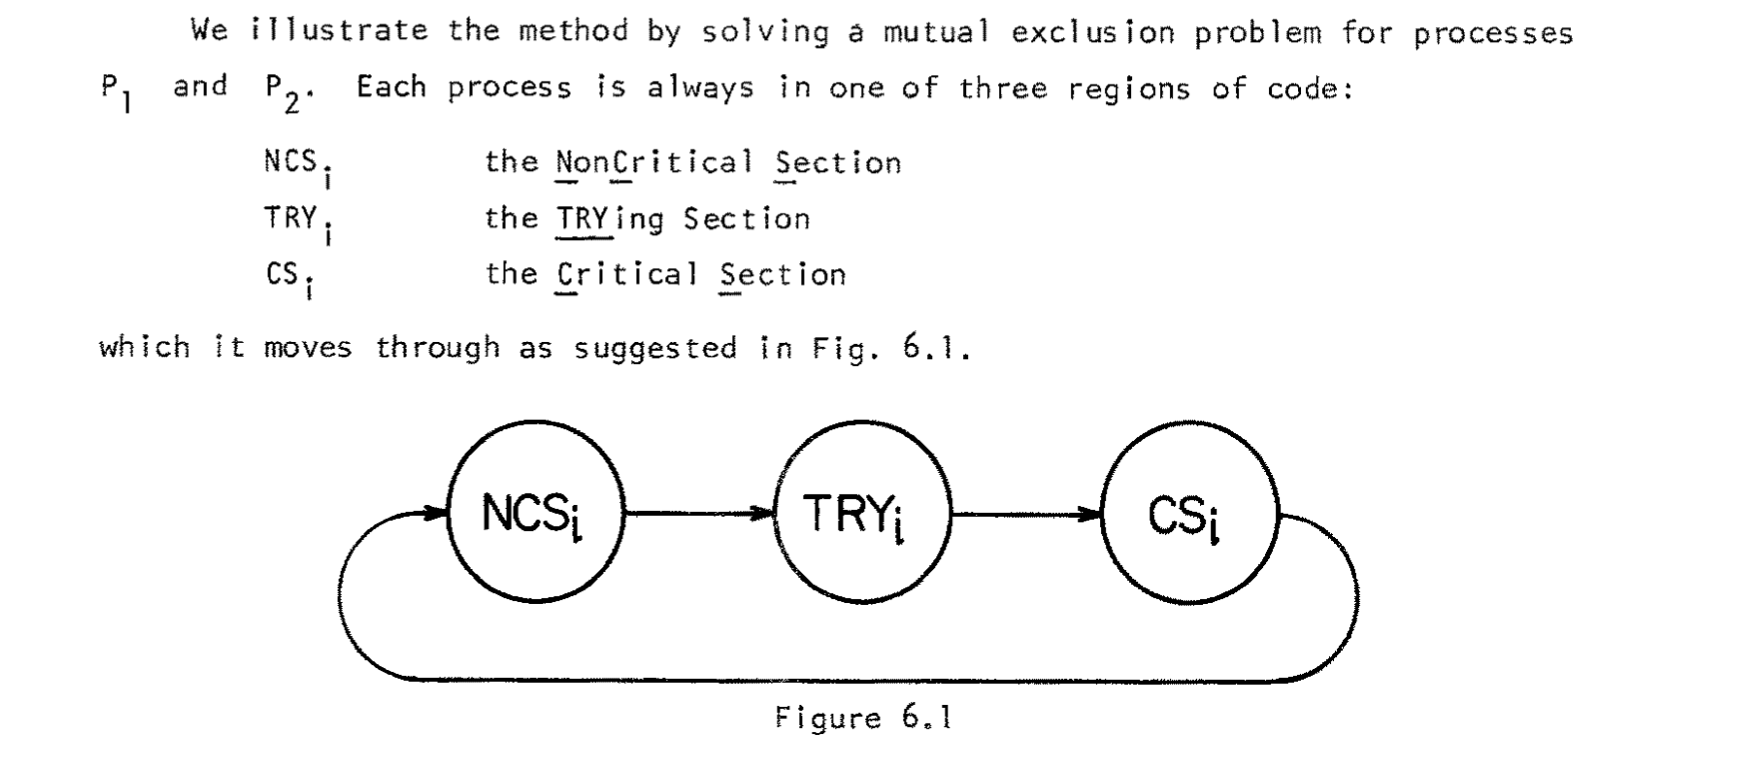
\includegraphics[scale=0.4]{images/mutex_processes.png}
\end{center}
and they give the specification of the mutual exclusion problem in CTL as follows:
\begin{center}
    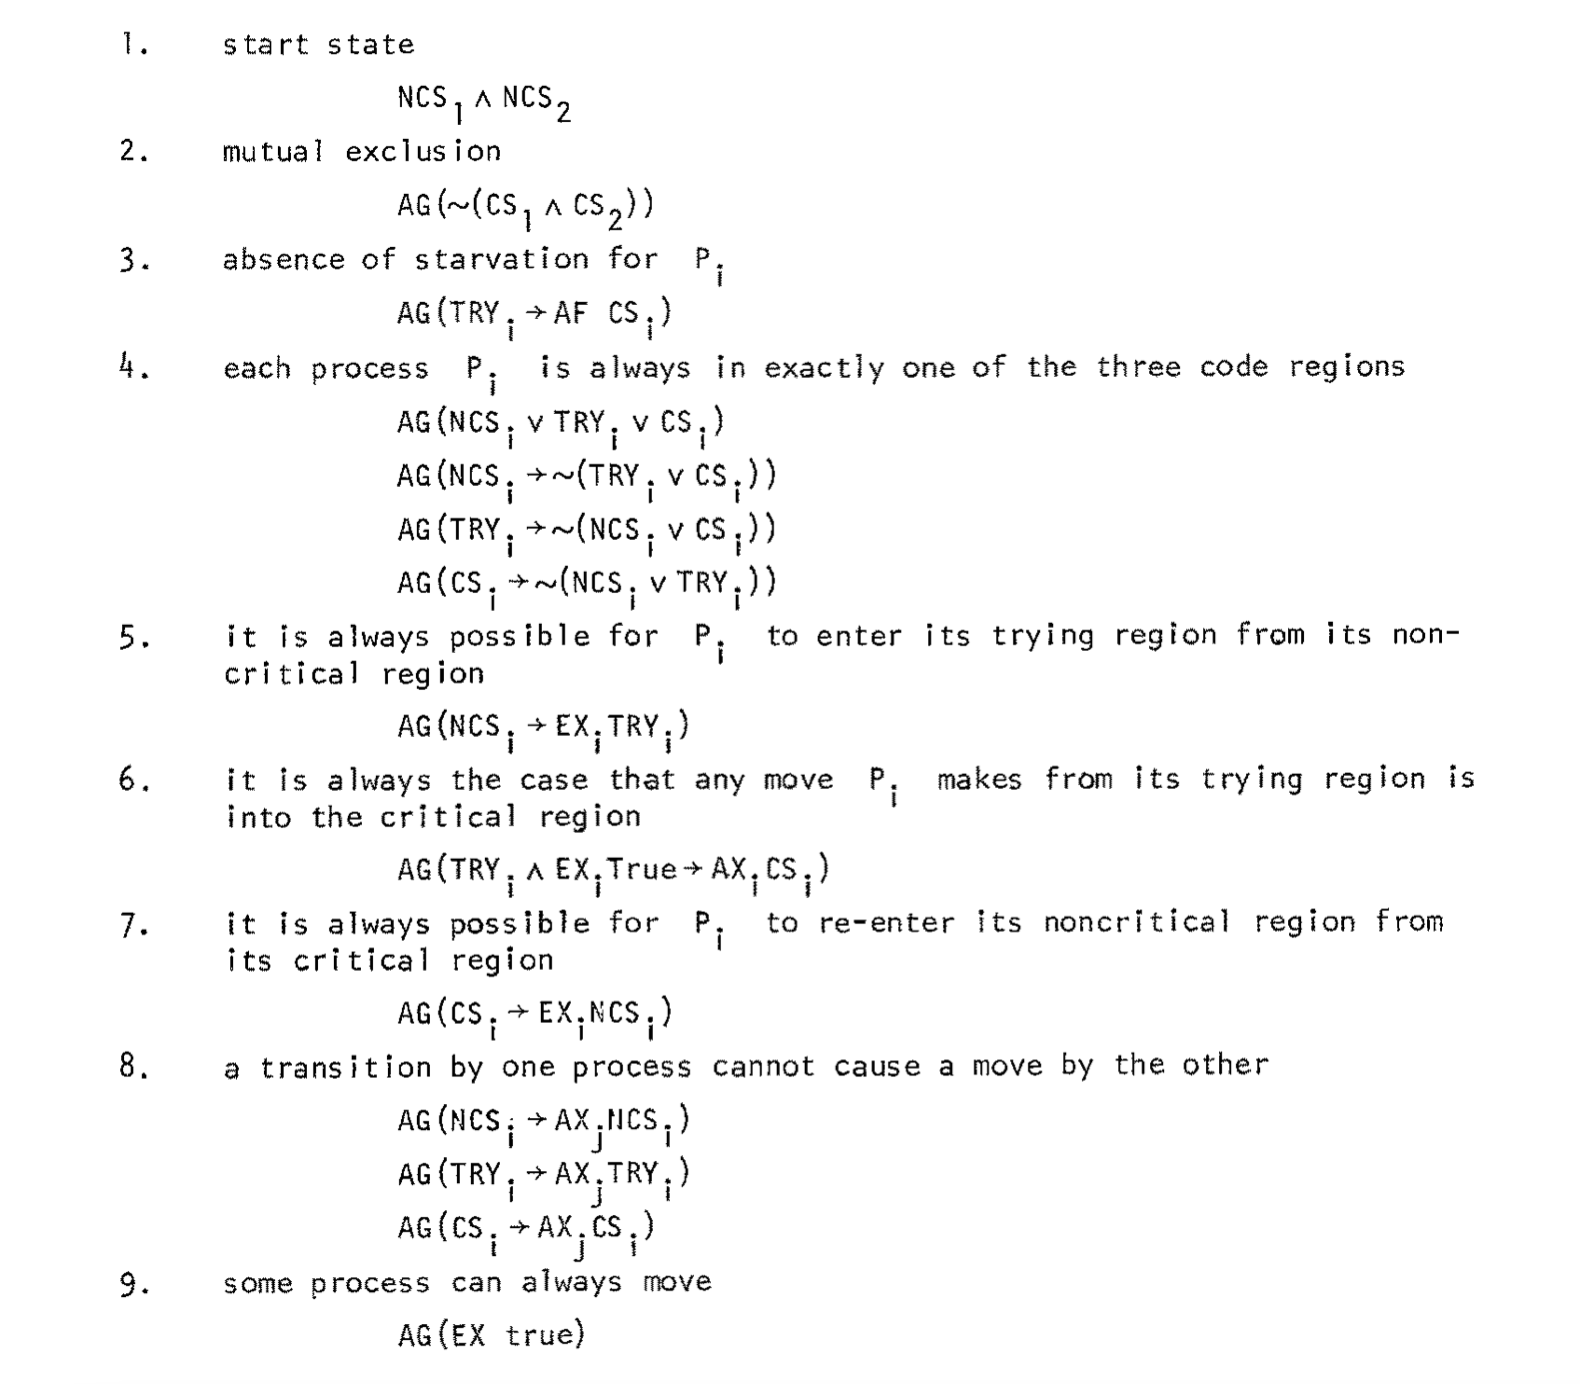
\includegraphics[scale=0.3]{images/mutex_spec.png}
\end{center}
From this they then construct the tableau $T$ using their decision procedure:
\begin{center}
    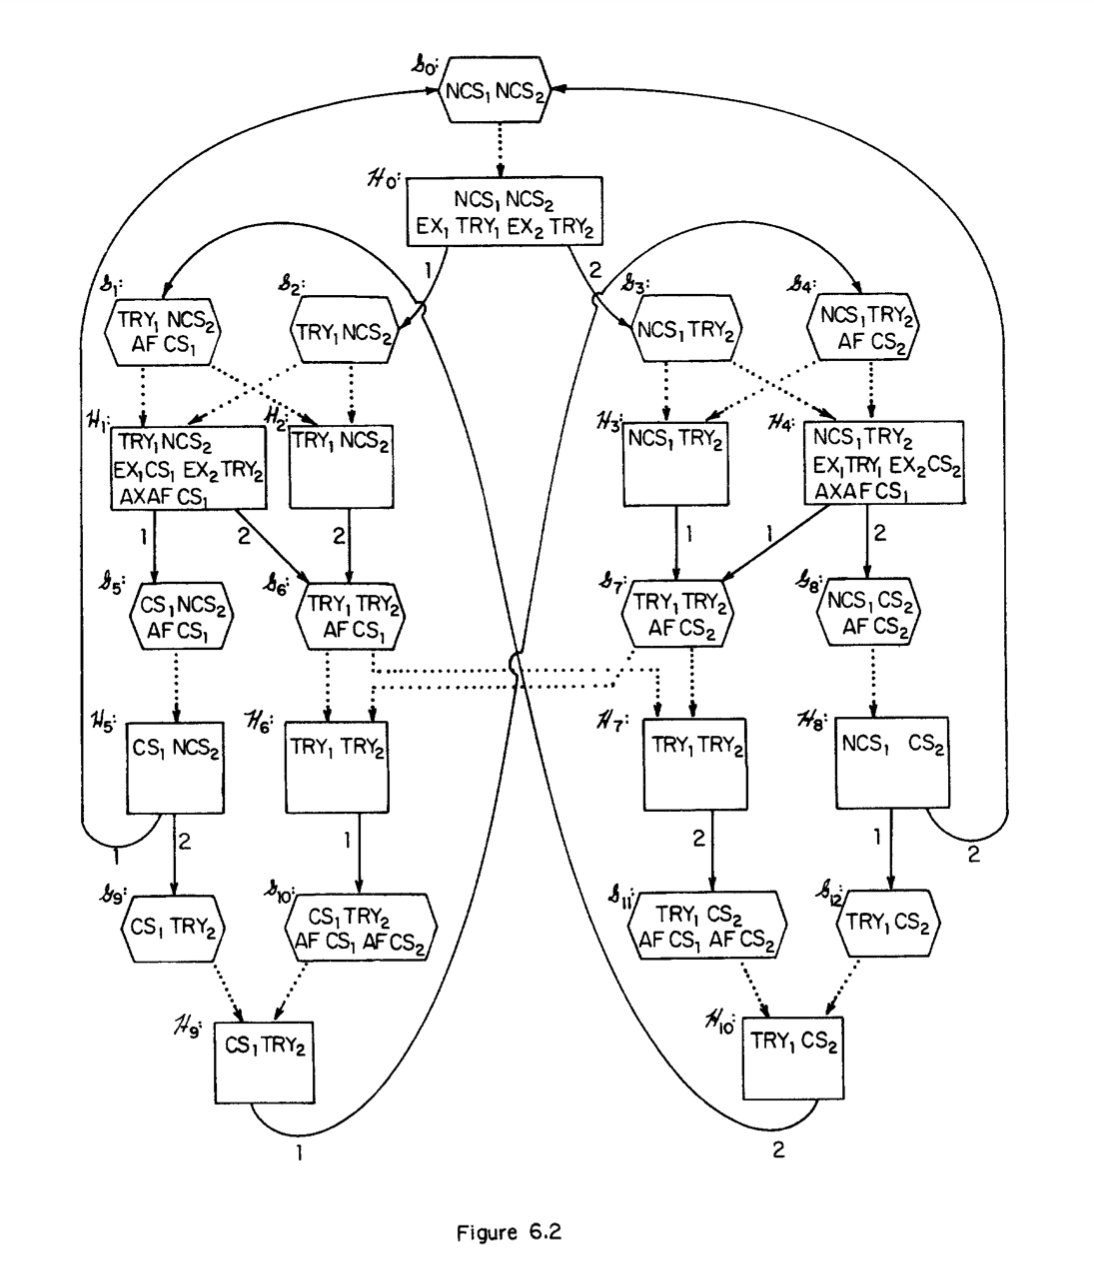
\includegraphics[scale=0.4]{images/mutex_tableau.png}
\end{center}
and then from $T$ they extract a finite model of the global program behavior:
\begin{center}
    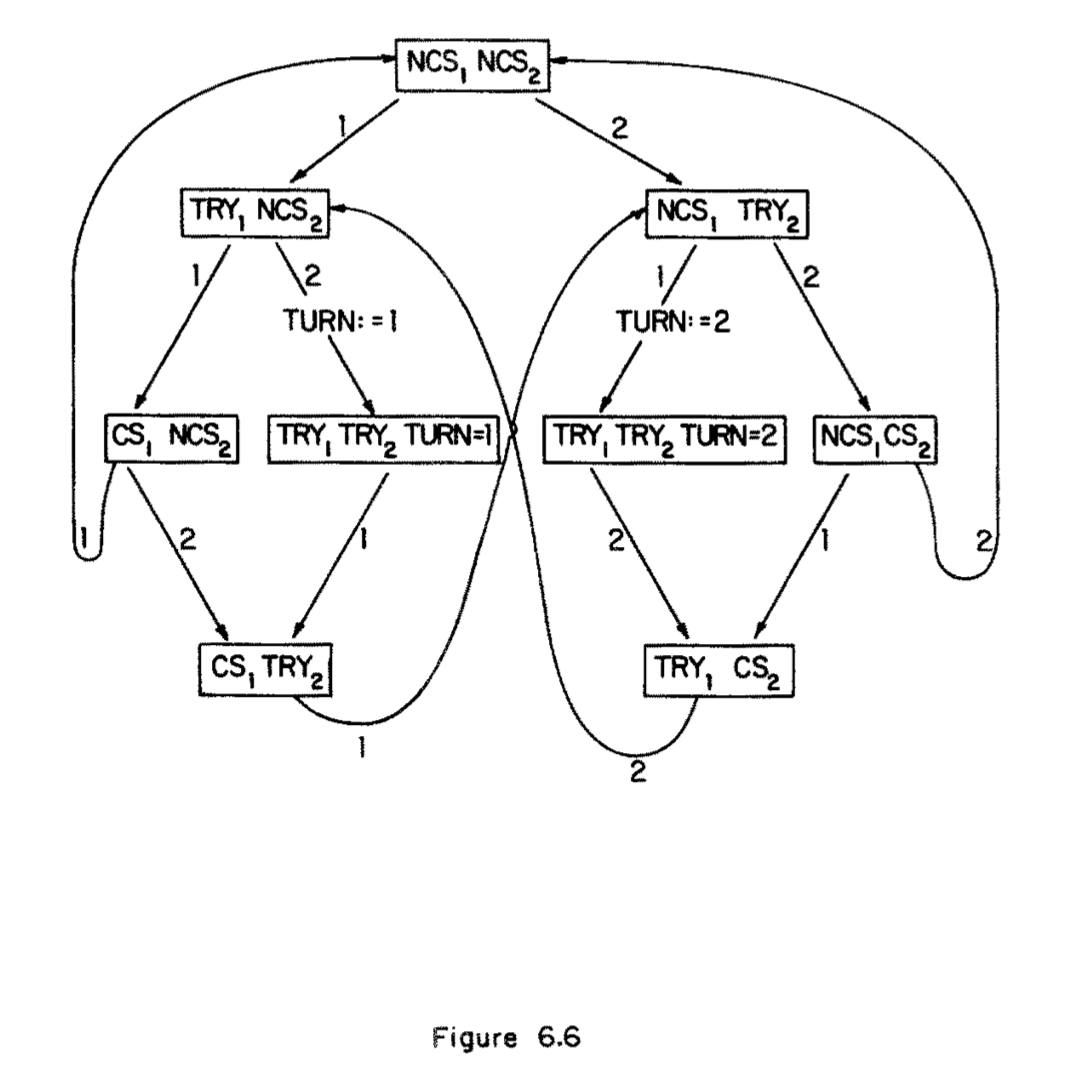
\includegraphics[scale=0.4]{images/mutex_model.png}
\end{center}
Note that they manually introduced an auxiliary variable $TURN$ in order to distinguish states $H_6$ and $H_7$ in the tableau, which carries over into the extracted model. After constructing the model representing the global program behavior, they then extract ``skeletons'' for each individual process, which they seem to describe in a somewhat ad hoc manner i.e. they don't seem to provide a formal algorithmic procedure for this. Note that this is pointed out in \cite{2001attie}, which appears to give a more formal treatment of this extraction procedure. The final, extracted skeletons for process $P_1$ and $P_2$ are shown as follows:
\begin{center}
    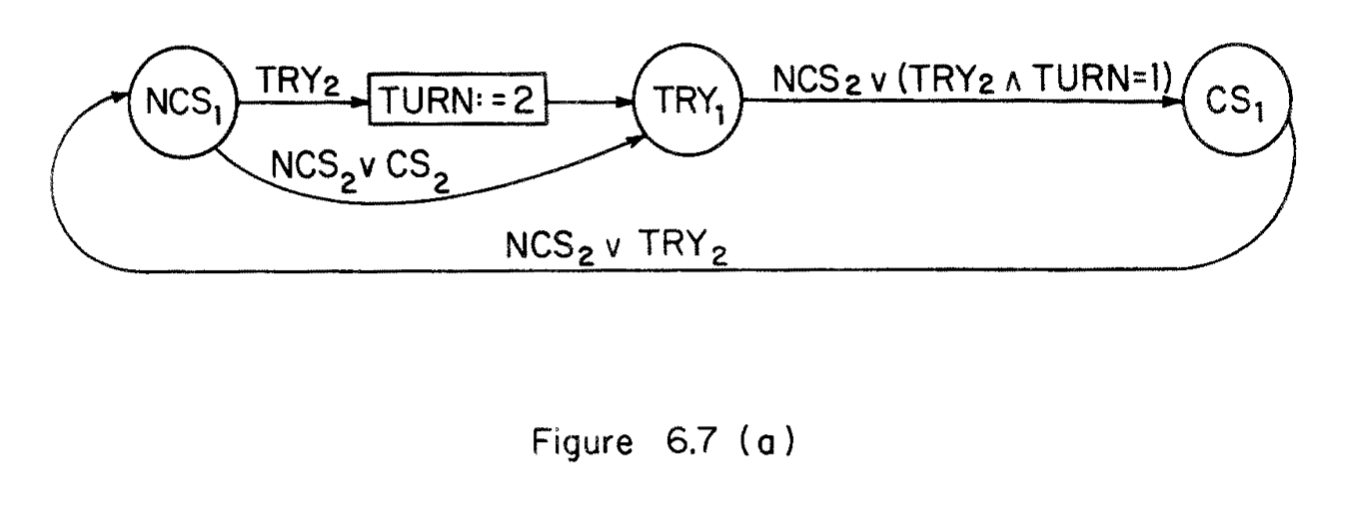
\includegraphics[scale=0.3]{images/mutex_p1.png}
\end{center}
\begin{center}
    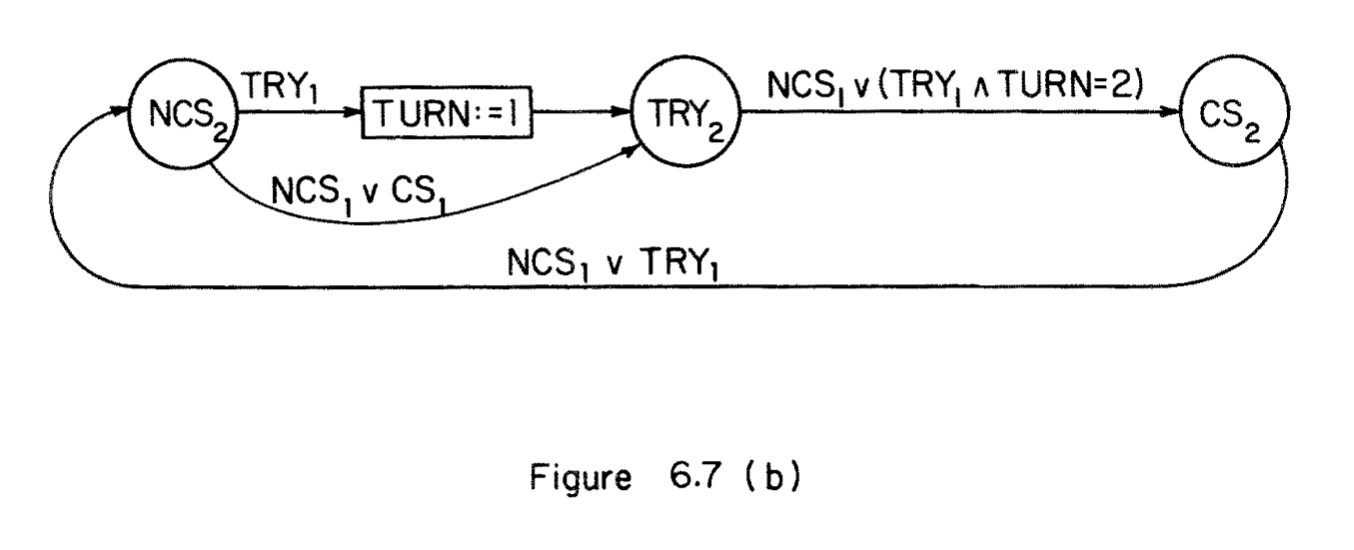
\includegraphics[scale=0.3]{images/mutex_p2.png}
\end{center}

% \bibliographystyle{plain}
\bibliographystyle{apalike} 
\bibliography{../../references.bib}

\end{document}